\songchapter{H}

%%%%%%%%%%%%%%%%%%%%%%%%%%%%%
\songsection{胡吗个}	\index{H!humage}

%%%%%%%%%%%%%%%%%%%
\subsection{人人都有个小板凳, 我的不带入二十一世纪}

\begin{figure}[htp]
	\begin{center}
	  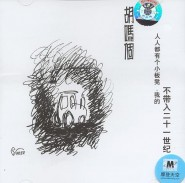
\includegraphics[scale = 0.80]{h/humage/renrendouyou}
	  \label{fig:renrendouyou}
	\end{center}
\end{figure}

\begin{songs}{}
  \beginsong{部分土豆进城}[index={部分土豆进城}]
	三月城市森林	\\
	我栖于树枝低檐	\\
	自己不筑巢	\\
	自己不种稻	\\
	替喜鹊看门	\\
	替黄鹂担粪	\\
	替老鹰带小孩	\\
	替花鸽送煤	\\
	以获取两只虫子度日	\\
	\vspace{2ex}
	隔壁住着一个怪怪的没有恶意的文化人	\\
	他说我勤劳勇敢善良朴实没有欲望	\\
	他拿出一本写了很多字的练习本给我看	\\
	又放一些不太好听很吵的歌给我听	\\
	他说那是在赞美我们	\\
	他说他就是我们	\\
	可却要把笑容垫在屁股下面的椅子上	\\
	又提到虚伪什么的	\\
	还说了一些城市的坏话	\\
	好多词我都听不太懂	\\
	只好歉歉地歉歉地说	\\
	这个我说不好 \hspace{5mm} 这个我实在说不好	\\
	这个我说不好 \hspace{5mm} 这个我实在说不好	\\
	这个我说不好 \hspace{5mm} 这个我实在说不好	\\
	这个我说不好 \hspace{5mm} 这个我实在说不好	\\
	\vspace{2ex}
	屋顶上的那只大花猫	\\
	它有福气 \hspace{5mm} 有阳台	\\
	可以抱着这个城市的户口整日睡觉	\\
	真想把它娶过来 \hspace{5mm} 摇身一变 \hspace{5mm} 上街去	\\
	看到一个二层的小洋楼	\\
	就好像刚盖的新房	\\
	我竟楞楞地楞楞地走了过去	\\
	把门的大姐递给我一张手纸	\\
	说 \hspace{5mm} 三毛钱一位	\\
	可是我的外地口音啊	\\
% 	可是我的外地口音啊	\\
% 	可是我的外地口音啊	\\
% 	可是我的外地口音我的外地口音啊	\\
% 	可是我的外地口音我的外地外地口音啊	\\
% 	可是我的外地口音外地口音啊	\\
% 	可是我的外地口音啊	\\
% 	可是我的外地口音我的外地口音啊	\\
% 	可是我的外地我的外地口音啊	\\
% 	可是我的外地口音我的外地口音啊	\\
% 	可是我的外地我的我的外地口音啊	\\
% 	可是我的外地口音我的外地口音啊	\\
% 	可是我的外地口音我的外地口音啊	\\
% 	可是我的外地我的外地口音啊	\\
% 	可是我的外地我的外地口音啊	\\
% 	可是我的外地外地口音啊	\\
% 	可是我的外地外地口音啊	\\
  \endsong

  \beginsong{到四道口换26路——我的忧伤难以启齿}[index={到四道口换26路——我的忧伤难以启齿}]
	桌子间还有缝隙	\\
	一些人面对面或者背靠背	\\
	这是办公室	\\
	墙上贴着制度表 \hspace{5mm} 与工资有关	\\
	大家才不会到班太晚	\\
	如果你从门外进来	\\
	你就首先会看见我们的女同事	\\
	她们花枝招展 还嫌自己不够	\\
	而我那儿光线实在太暗	\\
	你知道我的办公桌是价值两万的吗?	\\
	你知道洗手间离我直线距离仅有3米远吗?	\\
	你知道我对面的石英钟每天慢20秒吗?	\\
	你知道 \hspace{5mm} 你知道	\\
	我这些忧伤实在难以启齿	\\
	\vspace{2ex}
	不知什么时候我开始热衷于打电话	\\
	我现在是电话迷	\\
	有时候 \hspace{5mm} 仅仅是趴在桌上	\\
	摘下听筒我就会喋喋不休	\\
	随便找个号码一拨	\\
	对方是个女孩	\\
	我说我是越南人吗个	\\
	(...?) 门口见	\\
	很是兴奋 \hspace{5mm} 左眼老跳	\\
	\vspace{2ex}
	刚撂下电话又来了个电话 \hspace{5mm} 还是个女孩 \\
	她说她要找秦勇(?) \hspace{5mm} 我说他不在她就哭 \\
	我说你别哭了你千万别哭 \hspace{5mm} 她还是哭	\\
	我说你是真的还是假的 \hspace{5mm} 她就不哭了	\\
	\vspace{2ex}
	尾顶上的老鼠换了一拔又一拔	\\
	有人写了份辞职报告	\\
	嗯 \hspace{5mm} 说是去了兰州	\\
	仅仅是 \hspace{5mm} 为了那儿的一碗拉面	\\
	他们口口声声为我们的留守者的明天祝福 \hspace{5mm} 即使庸俗	\\
	后来又有几个人从门缝里挤了进来	\\
	格外小心翼翼	\\
	我每天都还在坚持着上班下班	\\
	兜里揣着月票	\\
	在四道口换26路	\\
	哎 \hspace{5mm} 明天还是自己找个女朋友去吧	\\
	光看别人的	\hspace{5mm} 也不好意思	\\
  \endsong
\end{songs}
